%===================================== CHAP 7 =================================

\chapter{Phase 3: Final Requirements and Finishing Up} 
\label{chap:7}
\label{chap:phase3}
The primary targets for the third and final phase of this thesis were to implement additional requirements, complete the artefact as a general multi-user framework to serve as a foundation for future development and analyse user test data. The following sections will describe changes due to Covid-19, development decisions and implementation, as well as an evaluation of this phase's artefact.                 


\section{Planning and Changes}
\label{section:planningandchanges}
Phase 3 was originally meant to contain changes and finishing touches based on the feedback received during phase 2. However, just as the main testing was about to begin, Norway took measures to limit spread of Covid-19 (see section \ref{section:covid19}), effectively preventing us from going through with the original plans for this phase. Coupled with an enforced work from home situation, the plan needed to be changed drastically. Primarily, some triage had to be done as to figure out which parts of the application were the most necessary for remote data gathering. Since the application is a proof of concept, it was never that important that it ran without supervision, or that multiple server instances could be run at the same time, since we were always present to run the tests and could manage all of this manually. Now that could no longer be assured. This lead to some significant changes in the planned schedule, and more features needed to be developed. A brief overview of the changes can be seen below.

\subsection{Changes}
\begin{description}
    \item [Change 1]\hfill \\
    Support for multiple concurrent rooms must be made. 
    \item [Change 2]\hfill \\
    Artefact must be changed to an executable file for end-users so it works with minimal or no input from developers.
    \item [Change 3]\hfill \\
    Features need to be complete and usable, or potentially removed if their unfinished state interferes with normal use of artefact.
    \item[Change 4]\hfill \\
    Modified research questions, as the new circumstances made some of the difficult to answer properly.
\end{description}

\subsection{Changes to Research Questions}
As a direct result of the Covid-19 situation, it became unfeasible to complete the research question looking into the difference between collaborating with a seeker compared to a counsellor, as it was impossible to set up a day for testing the scenarios properly. In order to thoroughly answer this research questions, we concluded we needed more people, and time to test with multiple combinations of seekers, counsellors and experts. As such, secondary RQ1 will not be answered in a way we had hoped to. See \textit{Future Work} in section \ref{section:futureWork} for more on this.

On the other hand, the new circumstances paved the way for an additional research question. During a discussion held with IMTEL and NAV, a need to figure out what parts are essential for remote career guidance to work was expressed. Thus, a new research question (secondary RQ2) was drafted, see section \ref{RQ}, with the aim of assessing essentials needed for collaborative VR in order for it to be applied effectively as a remote career guidance tool. 

A revised plan for this phase was drafted to handle the new situation regarding the Covid-19 restrictions and adapt to the changes of the research questions. The new plan included testing with NAV clients remotely, online seminars and testing with experts from NAV and Kompetanse Norge. See section \ref{section:evalPhase3} for more details.    

As such, the new topic regarding remote career guidance could be integrated seamlessly into the paper with only some minor adjustments to surveys and plans. Therefore, work began on stabilising features in the application so remote guidance could work smoothly. With the final features in place, the survey could be updated to find out which of them were essential, and whether any features were missing that we had not considered.


\subsection{Final Requirements}
As outlined in section \ref{section:planningandchanges} this phase saw changes to the artefact and past plans. The requirements outlined in bold are additions for this phase.

\begin{enumerate}
  \setlength\itemsep{0em}
    \item [\textbf{F1}] The applications must allow multiple players to join the same scene.
    \item [\textbf{F2}] Interactable objects must be serialised and and synchronised over the network.
    \item [\textbf{F3}] A player shall be represented as an avatar with corresponding movement from the real world to the VR world.
    \item [\textbf{F4}] The application must offer the option of using VR equipment or desktop mode (mouse and keyboard) for interaction.
    \item [\textbf{F5}] The application must contain a scene with tasks enabling collaborative learning.
    \item [\textbf{F6}] The multiplayer component must be generalisable and scalable to work with other NAV applications.
    \item [\textbf{F7}] The application must be a virtual workplace with multi user functionality.
    \item [\textbf{F8}] Users should be able to communicate through integrated voice chat functionality.
    \item [\textbf{F9}] VR users should be able use tool(s) to mark or pinpoint objects or locations.
    \item [\textbf{F10}] \textbf{The application must support a lobby system allowing multiple concurrent instances of an application to run simultaneously}.
    \item [\textbf{F11}] \textbf{A room instance should support at least sixteen VR or desktop users to join.}
    \item [\textbf{F12}] \textbf{A distributable executable file must be made available to users.}
\end{enumerate}




\subsection{Development Decisions}
While the previous phase focused on creating a fully functional multi-user collaborative workplace by implementing network functionality into a car mechanic workplace, phase 3 is about adding remote usage possibilities in the existing artefact while finishing up prioritised features.  


\subsubsection{Remote Application Use}
In order for the virtual internship to be used successfully in remote circumstances, it was decided that the artefact needed updates to the limited \textit{Launcher} logic. Architecture, setup, network related methods and callbacks, as well as optimisation settings needed an overhaul so that clients could seamlessly host, create and join instances of different applications (rooms). The launcher logic should also include multiple selectable applications (scenes) so that it could serve as a foundation for future development and be utilised to demonstrate the basics of implementing multiple workplaces into one lobby.   

\subsubsection{Usability}
User experience have always been considered when developing the application, but it was mainly in relation to the VR aspect, and less focus was placed on other parts such as the user interface for the lobby. For the application to be used remotely by users, this phase's artefact should include a distributable file. Hence, more consideration towards the usability of the software had to be taken. A general rule of thumb while developing software is to have a goal that whomever (young digitally-skilled or elderly with little skill) should be able use it with as little support as possible. With that in mind the development must consider subjective objectives such as intuitiveness, ease of use, feedback, and efficiency to hopefully increase the overall satisfaction for the end users.



\subsubsection{Networking}
Due to the shift in focus for this phase, many possible challenges were discussed. One of them being an increased number of concurrent users. From previous phases the intention of the artefact was to accommodate collaboration mechanisms by allowing two or three users to work together (possibly more, but with an intended cap at six). Introducing a distributable file we decided that it should at least sustain sixteen concurrent users per room (application instance) to better accommodate different scenarios for remote career guidance. An increase in concurrent users of at least 150\%. 

The PUN2 framework we opted to use in development uses Photon Cloud to host the server-side of the application. Photon has several subscription plans for this, including a free \textit{Public Cloud}. That was the plan used in phase 1 and 2. At the time it was the obvious choice, being free and providing plenty of capability for the intended use. This plan supports up to 20 Concurrent Users (CCU), i.e., the number of users allowed to connect to the application, eighth thousand monthly activities and 500 messages per second per room. The other subscription plans \textit{Premium Cloud} and \textit{Enterprise Cloud} can handle 50.000+ CCU but has a cost of at least \$580 per month. After some network traffic calculations and discussion we decided the \textit{Public Cloud} could still satisfy our needs, but some restrictions in the code was needed to limit the number of users so that it does not exceed the CCU cap. 





\section{Final Artefact}
As the development came to a close, and the highest priority requirements were finished up, a final version of the artefact was created and prepared for testing. To be able to test properly, it is important that all testers experience the same artefact. By prioritising the features with the greatest impact on the overall experience, it is possible to create an artefact that captures the essence of the concepts presented in the paper. While not every desirable feature were implemented, the final artefact still stands as a usable proof of concept with a fully functional lobby system, app selection and a network synced VR workplace. Figure \ref{fig:finalArtefact} shows the car mechanic scene from the final artefact. A \href{https://www.youtube.com/watch?v=ZNnK4ohWSag}{\textcolor{blue}{YouTube}} video is found at \textcolor{blue}{\textit{https://www.youtube.com/watch?v=ZNnK4ohWSag}} showing the system in action.


\begin{figure}[]
  \centering
  \captionsetup{width=1\linewidth}
    \includegraphics[width=1\textwidth]{fig/phase_3/final/finalfinal.png}
  \caption{Screencaptures of the final artefact showing both VR users as avatars and desktop users as orange pointers.}
  \label{fig:finalArtefact}
\end{figure}



\subsection{Lobby Supporting Different Applications}
\label{section:lobbySystem}
Being a part of the larger collaboration project between IMTEL and NAV, it is natural for new projects to build on the older ones, as this one did. To further enable this process, considerable effort went into making sure the artefact is reusable and easy to expand further should the need arise to do so. As part of this, the starting screen of the application received updates, as seen in figure \ref{fig:phase3_lobby1}. All the elements in the user interface were redesigned to support multiple resolutions so that the layout adapts to it.  
We also included a new feature, where the user can select which application they would like to start as a mean to ease reusability and future development, seen in figure \ref{fig:phase3_dropwdown}. This allows future developers to effortlessly target any desired scene (or application) to be created as a public hosted instance on the server so that users can join. 
However, it must be pointed out that this does not serialise or network objects within the scene automatically. Players that join the room are synchronised, but every other interactable object requires some level of PUN2 networking implementation. 
    

\begin{figure}[H]
  \centering
   \captionsetup{width=.9\linewidth}
    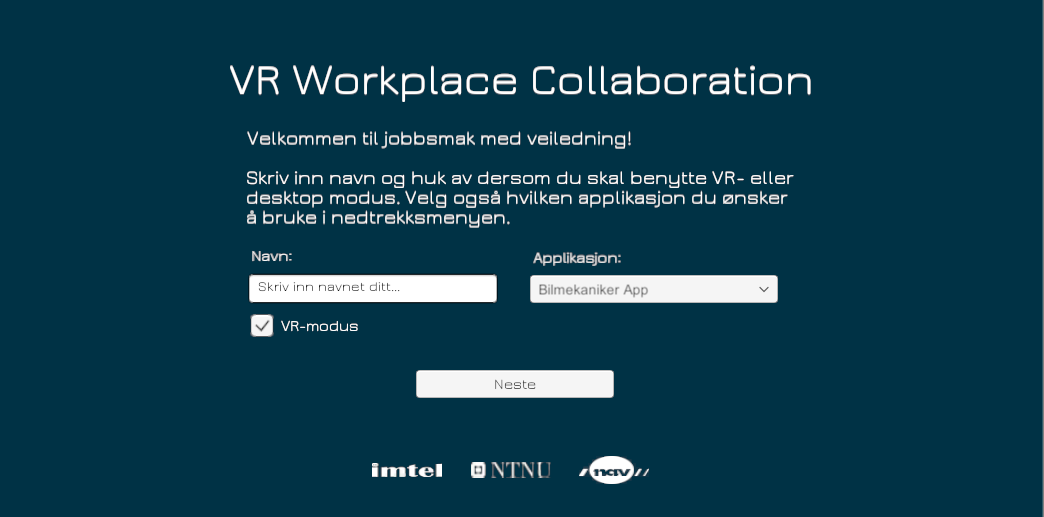
\includegraphics[width=0.9\textwidth]{fig/phase_3/implementation/Lobby1.PNG}
 \caption{The redesigned \textit{Launcher} screen the user meets after launching the application.}
\label{fig:phase3_lobby1}
\end{figure}



\begin{figure}[H]
  \centering
   \captionsetup{width=.4\linewidth}
    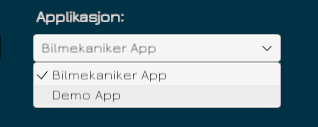
\includegraphics[width=0.4\textwidth]{fig/phase_3/implementation/LauncherDropdown1.png}
 \caption{Dropdown element for targeting launch of a specific application. }
\label{fig:phase3_dropwdown}
\end{figure}

Once a specific application is chosen in the dropdown and the \textit{Next} button is pressed the user is taken to a new \textit{Lobby} screen for the selected application as seen in figure \ref{fig:phase3_LobbyScene1}. Here the users have several options. First, the system automatically connects the user to the Photon network and once connected successfully it joins the corresponding lobby based on the application selected in the previous screen.    
Then the system fetches all the corresponding rooms (application instances) hosted on the Photon Cloud server. If none are found, meaning no rooms are active or being hosted, a simple textbox notifies the user that no rooms exist and that they can create their own. Otherwise, the rooms are listed in a scrollable list element, see figure \ref{fig:phase3_LobbyMultiRoomsSelectSmall}. 

\begin{figure}[H]
  \centering
   \captionsetup{width=.9\linewidth}
    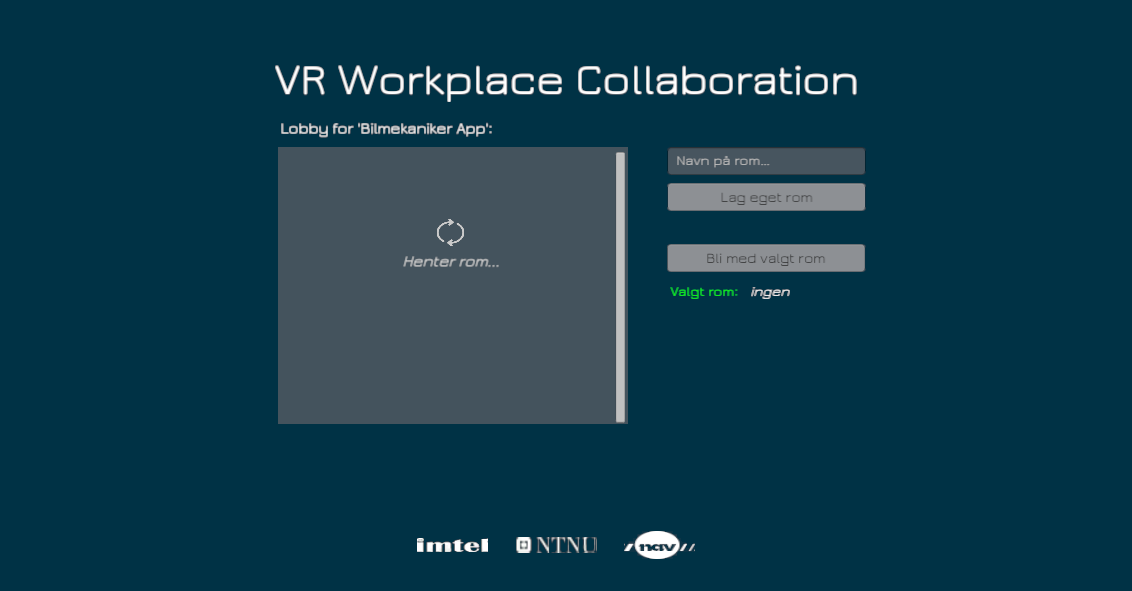
\includegraphics[width=0.9\textwidth]{fig/phase_3/implementation/Lobby2Fetching.PNG}
 \caption{Lobby screen for a selected application. In this instance the \textit{Auto mechanic app}.}
\label{fig:phase3_LobbyScene1}
\end{figure}

\begin{figure}[H]
  \centering
   \captionsetup{width=.8\linewidth}
    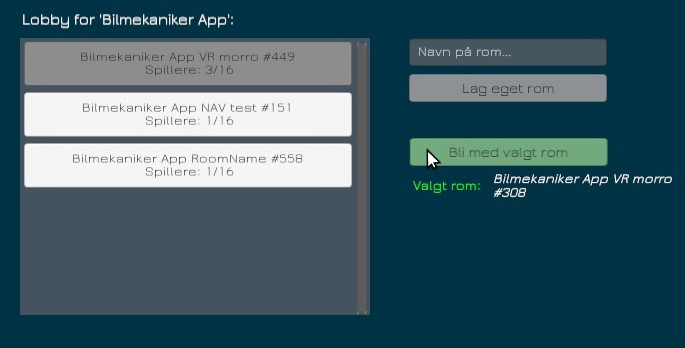
\includegraphics[width=0.8\textwidth]{fig/phase_3/implementation/Lobby2MultiRoomsSelectedSmall.jpg}
 \caption{Cropped screenshot of the lobby, listing hosted rooms and a user ready to join a selected room.}
\label{fig:phase3_LobbyMultiRoomsSelectSmall}
\end{figure}

The process of creating a room was to a large extent simplified (while ensuring functionality is kept) so that most users could perform the operation. Only a name for the room is required. It does not need to be unique, as that is accounted for in the code. Custom logic assigns a unique ID number to a room instance, which is then used as a key identifier when a user wants to join that room. Once a user successfully creates a room on the server, the client joins the room and their local player instance is instantiated. They are now the master client of the room. If they were to leave, and other users are connected to the room, the master client privileges are delegated to another user. Otherwise the room is closed. After the client has created and joined the room, a callback is made to all connected remote clients in the lobby and the room is added and displayed in the list of rooms. 

To join a hosted room the user only needs to select the desired one from the list by clicking on it and press \textit{Join selected room}. As a verification that the correct room is selected, a text string below the join button is updated with the corresponding room name, see figure \ref{fig:phase3_LobbyMultiRoomsSelectSmall}. Similar to creating a room, the process of joining is automated. The difference being there is no need to create it, just instantiate the client's local player instance. 

A player cap of 16 concurrent users are set for each room. The number of connected clients in a room are shown in the list of rooms along the name, type of application and ID. See figure \ref{fig:phase3_LobbyMultiRoomsSelectSmall} for an example.  


To demonstrate the new feature that allows multiple applications in the lobby system, a demo application was made. The dropdown menu allows the users to select different applications and see the new feature in action. It also serves to demonstrate how to implement a new scene for future developers who may use the lobby system. This aligns closely with secondary RQ4, as part of the challenge of implementing these features is that they must be general enough to work in a multitude of scenarios. Figure \ref{fig:phase3_demoApp} is a screenshot of the demo application scene. This is not the early demo from phase 1, but a new barebones scene used as an example of how to manage multiple applications in the launcher, primarily for the benefit of other developers.  


\begin{figure}[H]
  \centering
   \captionsetup{width=.9\linewidth}
    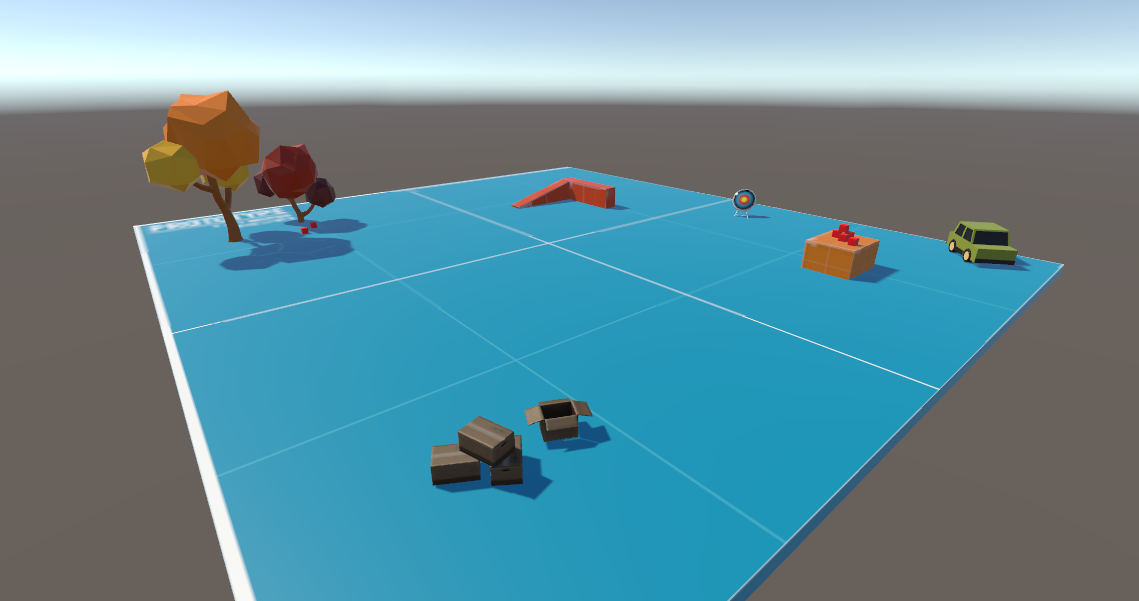
\includegraphics[width=0.9\textwidth]{fig/phase_3/implementation/demoApp.PNG}
 \caption{The example application with basic collaboration mechanism and networked integration.}
\label{fig:phase3_demoApp}
\end{figure}






\subsection{Improvements}


\subsubsection{Identifiable rooms}
In the preliminary stage of this phase the primary focus was to implement a functional lobby system as described in section \ref{section:lobbySystem}. To begin with, the rooms only had an identification number and the type of application as room name. The ID was set when the room was created. This meant the creator of a room did not know the ID and it was hard for other users to identify which room they were supposed to join. As such we improved the situation by allowing the users to enter a custom name for the room so that other users could identify the room by its name.   


\subsubsection{Custom keybindings}
As mentioned in the previous chapter (see section \ref{section:covid19}) we had gotten Oculus devices to support our work from home. We therefore added custom controller binding settings so that features such as laserpointer were supported for Oculus Touch controllers.   



\subsection{Usability}
As a measure to increase the users' opinions about subjective objectives related to the artefacts usability we considered and added different heuristics. 

First, we added symbols and status text so that the user has visibility of the system status. As an example the lobby displays a loading symbol and appropriate text in the room list while it is fetching data, seen in figure \ref{fig:phase3_LobbyScene1}.  
To prevent error by the user, some buttons are disabled until the user fulfils the requirements. In our solution the user needs to enter a name for the rooms before the \textit{Create own room} button becomes active and clickable.
The use of consistent elements such as colour scheme, size of buttons, text font and other mechanisms were also adapted. For example a mouse hovering over a button yields the same green colour overlay for all buttons to signal that it can be clicked. See figure \ref{fig:phase3_LobbyMultiRoomsSelectSmall}. 



\subsection{Challenges}

\subsubsection{Corrupted Prefabs}
The work from home environment presented some issues that were not expected. When work was done at the lab, the computers were kept up to date, programs were updated and things ran smoothly. When setting up at home, a fair bit of time was spent correctly setting up VR headsets on home computers, and importing the project files onto a new install of Unity. One of the issues was related to Unity prefabs and Blender files. During an import, several prefabs stopped working properly due to a lacking blender install. References to these prefabs broke, models did not show up as intended, and related networking components stopped working. 

As it turns out, \textit{.blend} files open in Blender in the background, and are exported as \textit{.fbx} files. But even when blender was installed on both computers used during the work from home period, there were still issues with certain \textit{.blend} files not being properly exported. Something about these files in particular must have used a newer function of Blender, as they were finally solved when the Blender version of the second computer was completely reinstalled to make sure the newest version was present on both computers. 



\subsubsection{GameObject tag - NullReferenceException}
During the development on a distributable executable file we experienced a bug in the build process. The application worked as expected when running it from the editor, but running it from the executable after the build process we would encounter a \textit{NullReferenceException}. This exception is raised when the system is trying to access a reference variable which does not refer to anything. It turns out if a tag is removed from the tag index, Unity will not see this change and the build file will try to access a variable which does not exist. In the application we used methods to get GameObjects by their tag, which was what raised the error. After much debugging the issue was solved by simply restarting Unity so that references and metadata was updated.  


\subsection{Unimplemented Features}
Due to the unexpected situation and the corresponding changes, some features that were wanted were not implemented. 

\subsubsection{Speech Indicator}
As mentioned in the previous chapter (see section \ref{section:phase2visibility}) some users have difficulty identifying who talks and when. One idea was to add speech indicators on avatars which is visible when a user talks in the application as a means to aid the visibility of speech amongst both VR and desktop users. Figure \ref{fig:phase3_speech} shows how such indicators might look.

The addition of speech indicator would be beneficial for the workspace awareness of the users in cases where there are more than two users at the same time. If users have trouble identifying who is currently speaking, the elements of identity and authorship (see table \ref{table:awarenessPresent}) are not reinforced enough. This negatively affects the workspace awareness of the user and, as a result, the overall experience suffers.


\begin{figure}[H]
  \centering
   \captionsetup{width=.6\linewidth}
    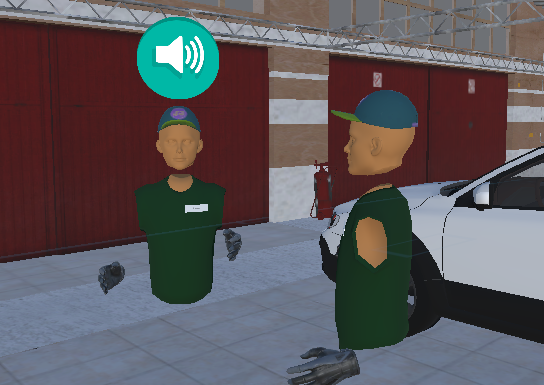
\includegraphics[width=0.6\textwidth]{fig/phase_3/implementation/speechIndicator.PNG}
 \caption{An example of how a speech indicator might look.}
\label{fig:phase3_speech}
\end{figure}


\subsubsection{Synchronised finger movement}
A discussed, but not implemented feature was the synchronisation and networking of the animated hands that Steam VR provides. While the hands of the user is correctly tracked and displayed to other users, the fingers are set in a static position. A user is able to see their own fingers move, but these animations are not played for other users.

When weighing the pros and cons of the feature, simplification of communication (see table \ref{table:awarenessActivity} is the concept that weighs most heavily. Deictic gestures are some of the most basic forms of communication, and any feature strengthening the users ability to communicate is worth considering for implementation. When prioritising different features, finger movement was not considered as important as other aspects of the artefact. To begin with, the avatars as they are now are not accurate or realistic, with missing limbs and little to no animation on the head. The direction, position and rotation of the hands were thought to serve satisfyingly as a representation of deictic gestures. Therefore finger movements were considered unnecessary for the current implementation, but may be considered later in the IMTEL project life cycle.



\section{Third Evaluation}
\label{section:evalPhase3}
While evaluation turned out to be more difficult than anticipated, tests were still able to be performed with some effort. As planned, tests with  users remain the primary source of data, but the new circumstances placed further importance on expert evaluation to garner additional data sets. Table \ref{table:dataGatheringSchedule} shows how and when data was gathered for this phase, which began with video conferences in April 2020. 


\subsection{Remote User Tests}
Since tests could no longer be performed at the lab or at the offices of NAV, they had to be adapted to fit the new circumstances. That meant finding testers who were available who also had VR gear at home. This turned out to be somewhat difficult, and a significant amount of time was  spent finding testers so that the project could finish as planned. Due to the collaboration with NAV, the task of finding suitable testers could be at least partially delegated to our collaborators at NAV. Since this would take an undetermined amount of time, time could be spent finishing up other aspects of the artefact that needed work or more polish to ensure the best result.

Finding job young seekers willing to participate turned out to be very difficult. A combination of lacking VR equipment, insecurity and no obligation to attend meant some job seekers first wanted to participate but ended up withdrawing from the testing. Due to the new circumstances, the amount of testers was drastically lower than initially planned for, so the methodology of testing had to be adjusted as well. As a consequence, these tests were conducted remotely over the internet using video conference tools and the remote guidance opportunities built into the artefact for this phase. Furthermore, more focus was placed on the qualitative data with additional quantitative data to support it, to make sure the samples obtained were useful and thorough. In late May, with testers finally secured, testing was conducted as planned. Although the amount of primary target testers were low, we had to proceed as they were the only ones available.   

Table \ref{table:dataGatheringSchedule} shows that large parts of April and May was used to prepare for and conduct video conferences and interviews. With the new restrictions in place, the importance of these interviews were further highlighted. By sourcing a template interview guide from another student at the IMTEL and altering it to suit our needs, we could relatively quickly create a high quality interview guide that would touch upon the subjects most important to us. The interviews needed to strike a good balance between length, content and accessibility. Compared to earlier interviews and discussions with users, there was definitely a barrier present when communicating via video conferences that meant conversations were less natural. As such, the interview guide had to maintain a high quality to properly extract the information that was needed. Were the conversation too long or the subject too dry or esoteric, the interest of the respondent might falter, leading to potentially poor data.

The interviews mostly took the shape of semi-structured interviews, which would allow on the fly adaptation if interesting topics sprung up. It also allowed for unsuited pr previously covered topics to be skipped when needed. Room was also left open for the respondents to discuss topics they felt were interesting and relevant to the research. Due to the situation, all of the interviews were conducted with a guidance counsellor from NAV present, which helped keep the conversation going, as the job seeker and counsellor were able to discuss their previous experiences with career guidance compared to this new way of career counselling.

\subsection{Expert Evaluation}
\label{section:phase3_expertEval}
While work was underway in securing testers for the planned remote guidance tests, other avenues for feedback were also pursued. Due to the special circumstances, there was some concern that enough test data could not be secured. By working with various collaboration partners of IMTEL, we could present the project and garner feedback and opinions from experts in the fields of career guidance and mentoring. While this alone is not a satisfactory type or amount of data, it is helpful to see their opinion on what we have made, particularly for the research questions that pertain to remote guidance, i.e., RQ2 and RQ3.

This data was primarily to be gathered using Microsoft Forms, where a survey was created over the course of multiple iterations. A copy of this form can be seen in appendix \ref{appendix:phase3}. Microsoft Forms was selected as it was suggested by the our advisers and complies with concerns regarding general data protection rules (GDPR), as well as being a platform all NTNU students have access to.

The largest opportunity for expert feedback happened in late April, where a possibility presented itself for a presentation and discussion with NAV and Kompetanse Norge, a directorate of the government department of education. While their field of expertise is primarily focused on the education and re-education of adults rather than young job seekers working with NAV, their expertise in the field of career guidance could be useful nonetheless.
This opportunity was an academic forum about VR in training and guidance hosted via Zoom, a video conference tool. During the meeting we presented our thesis and the developed artefact. To ease the explanation we made a short video showcasing and demonstrating the potential and features of the artefact. The video is available on  \href{https://www.youtube.com/watch?v=ZNnK4ohWSag}{\textcolor{blue}{YouTube}} \footnote{https://www.youtube.com/watch?v=ZNnK4ohWSag}. 

The survey that was prepared for the final phase consisted of four main sections aimed at providing data related to our research questions. These sections included \textit{Decision Learning and Career Guidance}, \textit{Collaboration Mechanisms}, \textit{SUS - System Usability Scale} and \textit{Remote Guidance}. Since participants of the survey could have different experiences with the application (used it, watched the video etc.) the survey considered all such cases, branching to the correct sections depending of their experience and answers. 

The survey was employed after the meeting in an attempt to gain a secondary data source. From the about 50 to 60 people we interacted with, 14 chose to respond to the survey. While the amount of respondents was not entirely as high as hoped considering this was not an entirely random selection for participants, their status as a secondary data source mitigates this somewhat, as this data was always considered secondary to the data gathered from the primary target group, which would be of the qualitative sort. We did however remind the participants of the meeting after some days to take the survey but with little response. More answers were provided by chief advisers in the Norwegian automotive association, who have worked previously with the IMTEL lab on career guidance projects.    



\subsection{Analysis}
Due to the challenges regarding user testing as described above data was gathered through both semi-structured interviews and surveys. Interviews were completed with the primary target users (young job seekers and career counsellors). The amount of interviews was limited and as such we also conducted surveys with experts to support our data gathering.      


\subsubsection{Qualitative Textual Data Analysis}
To analyse the textual data from the interviews conducted we utilised the same method and procedure as previously used in section \ref{section:phase1Analysis}. See appendix \ref{appendix:phase3} for interview guide and answers. Using theme analysis we identified themes and  related refined sub-themes as seen in table \ref{table:phase3ThemeAnalysis}. Table \ref{table:phase3MethaphorsAnalysis} shows relevant metaphors found in the interviews for each participant, and table \ref{table:phase3SatisfactionAnalysis} presents the interviewees perceived value of the final artefact developed for this thesis and the underlying concept.


\begin{table}[H]
      \centering
        \begin{tabular}{ll}
        \toprule
        Theme & Sub-theme \\
        \midrule
       Positive effect & Engagement\\
        & Social skills \\\vspace{0.2cm}
        & Self-efficacy \\
        Ease of use & Intuitive\\\vspace{0.2cm}
        & Low threshold to get started \\
        Career guidance & Shared virtual environment\\\vspace{0.2cm}
        & Conversation starter \\
        \bottomrule
        \end{tabular}
        \caption{The identified themes and sub-themes from the analysis.}
        \label{table:phase3ThemeAnalysis}
\end{table}






\begin{table}[H]
\centering
\begin{tabular}{l|lllll}
                        & \#01      & \#02     &\#03    &\#04 & \#05\\ \hline 
Positive effect         & *          &*          & *        & *     &*\\ 
Cooperative presence    & *          & *         &          & *     &\\ 
Engagement              & *          & *         & *        & *     &*\\ 
Decision learning       & *          & *         &          & *     &*\\ 
Collaborative learning  &            & *         & *        &       &\\ 
User representation     & *          &           & *        &       &\\ 
Availability            &            & *         & *        &       &*\\ 
Gesticulation           & *          &           &          &       &*\\ 
Intuitive               & *          & *         & *        &*      &*\\
%Speech indication      &            &           &          \\


\end{tabular}
\caption{Identified metaphors/keywords from the interview data.}
\label{table:phase3MethaphorsAnalysis}
\end{table}


\begin{table}[H]
      \centering
        \begin{tabular}{llp{2.5cm}p{5cm}}
        \toprule
        Role & ID & Perceived value of the concept & Reason\\
        \midrule\vspace{0.2cm}
         Job seeker  & \#01 & High & Very positive in regards to teaching and showing how things work. You can physically show, instead of talking from outside the app.\\
         & \#05  & High potential & Yes, I definitively think so. Speaking from previous experience, [...] people motivate each other, and dare to do more, as they can't see other real people looking at them.
         \\\midrule \vspace{0.2cm}
        Career counsellor & \#02  & High & In a situation where geographic distances are challenging, the concept is very valuable. The multiplayer concept is very interesting.\\ \vspace{0.2cm}
        Career counsellor & \#03  & High & Has a lot of potential. Being able to communicate with VR headset on, being able to collaborate like that and being able to work with employers are good things. \\ 
        Career counsellor & \#04  & High & In regards to VR as a remote guidance tool it is a very cool way of reaching many people. I thinks multiple users can increase engagement. \\
        \bottomrule
        \end{tabular}
        \caption{Perceived value of the concept grouped according to the role of each interviewee.}
        \label{table:phase3SatisfactionAnalysis}
\end{table}

Unlike the previous phases we decided to include direct quotations from participants of the target group as it shows their exact language and helps to point out important points. 
The following quotes presented below are opinions of participants from the interview process which we found to be both of value and interest. They are translated from Norwegian to English and grouped in corresponding themes.

\vspace{0.2cm}
\noindent\textbf{Engagement}
\label{quote:engagement}
\begin{displayquote}
\textit{"I think VR creates engagement, because I see how gaming how affects how they collaborate and discuss to solve issues."}
\end{displayquote}

\begin{displayquote}
\textit{"Engagement definitely increases, I would say. It is based on what I said earlier about collaboration in a workplace, it becomes more serious."}
\end{displayquote}


\newpage
\noindent\textbf{Presence}
\begin{displayquote}
\textit{"I have not used VR multiplayer too much before, it has mostly been single-user or turn based multi-user. So I have limited experience, but I felt the presence of another VR user as an avatar during testing.  Movement, and what he was planning was understandable."}
\end{displayquote}

\vspace{0.2cm}
\noindent\textbf{Collaboration mechanism}
\begin{displayquote}
\textit{"A laser pointer is very handy for counsellors, and if a user is wondering about something then you can point at the problem specifically. "}
\end{displayquote}

\begin{displayquote}
\textit{"Voice communication worked really well. Obvious who said what."}
\end{displayquote}

\begin{displayquote}
\textit{"...when people are talking a small talk bubble could appear, I think it would be better, especially if you are more than two users at the same time."}
\end{displayquote}


\vspace{0.2cm}
\noindent\textbf{Ease of use}
\begin{displayquote}
\textit{"Downloading and getting started was easy. I think it was pretty clear and quite self explanatory."}
\end{displayquote}




\subsubsection{Quantitative Data Analysis}
The data from the expert evaluation process was generated through a survey made using Microsoft Forms. See appendix \ref{appendix:phase3} for the full survey and answers. To get meaningful and interesting information out of it, we used similar techniques as the previous analysis phases to manage, view and analyse the data. The survey mainly consisted of ordinal data types from likert scales, a few nominal data types from categorical questions and finally one interval data type for the age of the participants.  
A benefit of utilising Microsoft Forms as our survey tool is that the data was automatically organised into visual aids such as bar and pie charts. Using these and the analysis we were able to identify interesting findings. 
The survey had 17 participants (experts in respective fields) consisting of 10 women and 7 men, all within the age group  of 45-64 years. 


The participants experience with VR was generally low, with 64,7\% ranking it either \textit{Very low degree} or \textit{Low degree}, but this was to be expected as the use of VR in public sectors is not common. 35\% experienced (used) the application on their own computer before answering the survey, whereas 65\% saw the video presentation as mentioned in section \ref{section:phase3_expertEval}.  



Independent of their experience of the application there was common consensus amongst all participants in relation to various statements regarding career guidance and decision learning. Figure \ref{fig:phase3_SurveyValgkompApp} and \ref{fig:phase3_SurveyValgkompVideo} shows the answers to similar statements but adapted depending on whether they used the application or watched the video presentation. As evident from the bar charts most participants ranked statements \textit{High degree} or \textit{Very high degree}. The mean being \textit{High degree} with an average of 59\% ranked for figure \ref{fig:phase3_SurveyValgkompApp} and 60\% for figure \ref{fig:phase3_SurveyValgkompVideo}.

\begin{figure}[H]
  \centering
   \captionsetup{width=.8\linewidth}
    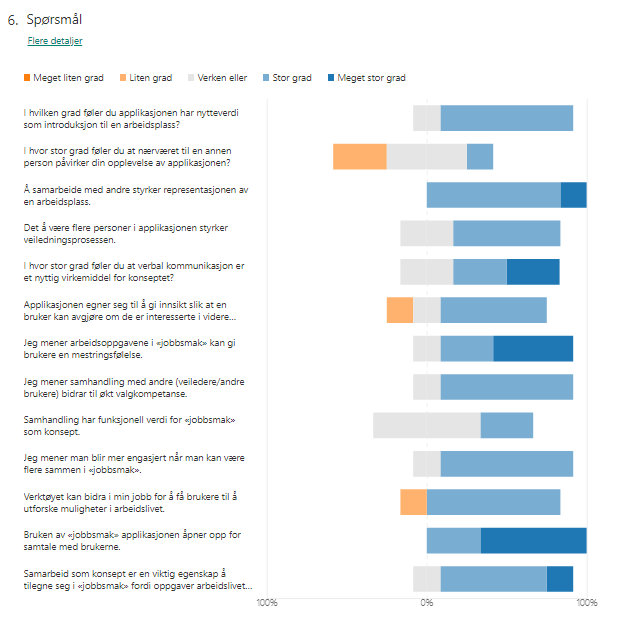
\includegraphics[width=0.9\textwidth]{fig/phase_3/survey/valgKompentanseApp.PNG}
 \caption{Bar charts showing participants who used the application ranking to various statements regarding career guidance and career decision.}
\label{fig:phase3_SurveyValgkompApp}
\end{figure}


\begin{figure}[H]
  \centering
   \captionsetup{width=.8\linewidth}
    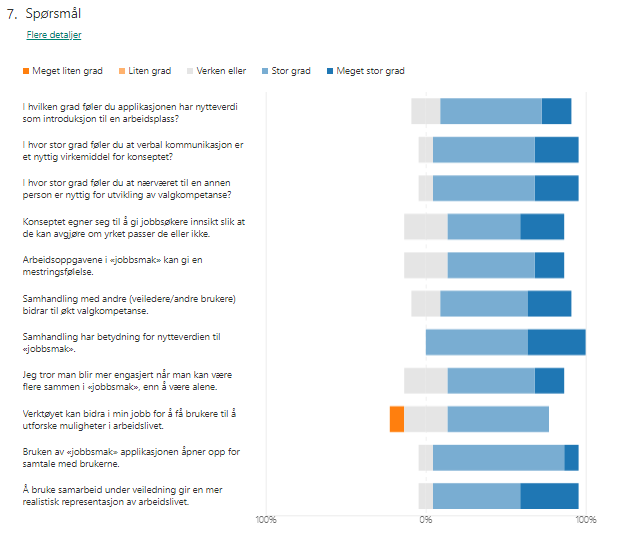
\includegraphics[width=0.9\textwidth]{fig/phase_3/survey/valgKompentanseVideoPNG.PNG}
 \caption{Bar charts showing participants who saw the video presentation ranking to various statements regarding career guidance and career decision.}
\label{fig:phase3_SurveyValgkompVideo}
\end{figure}






Most participants agreed that collaboration can contribute to decision learning in regards to career choice as seen in figure \ref{fig:phase3_SurveyCollaborationIncreased}. Here the mode was \textit{High degree} with 83.3\% of participants ranking it. However 16,7\% of participants were neutral in their opinion. This was the exact ranking received for another statement in regards to potentially increased engagement when there are multiple users present in the application, see figure \ref{fig:phase3_SurveyEngagementIncreased}. Interestingly, the participant were divided in how they experienced the feeling of presence affected the experience of the application as seen in figure \ref{fig:phase3_SurveyPrecenceIncrease}. Here the mode was \textit{Neutral} with 50\%. \textit{High degree} was ranked only 16,7\% whereas \textit{Low degree} was ranked 33,3\% of the time. A clear spread of data values, illustrating a difference in opinion between the participants.


\begin{figure}[H]
  \centering
   \captionsetup{width=.8\linewidth}
    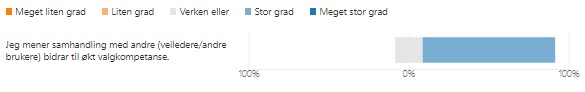
\includegraphics[width=0.9\textwidth]{fig/phase_3/survey/ValgKompAppSamhandlingOkt.jpg}
 \caption{Bar chart showing the distribution of how the participants ranked according to the statement: \textit{In my opinion collaboration with others (carer counsellor/other users) contributes to increased carer decision learning}.}
\label{fig:phase3_SurveyCollaborationIncreased}
\end{figure}

\begin{figure}[H]
  \centering
   \captionsetup{width=.8\linewidth}
    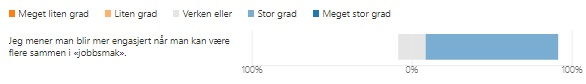
\includegraphics[width=0.9\textwidth]{fig/phase_3/survey/ValgKompAppEngasjement.jpg}
 \caption{Bar chart showing the distribution of how the participants ranked according to the statement: \textit{In my opinion the engagement increases when there are multiple users in the application}.}
\label{fig:phase3_SurveyEngagementIncreased}
\end{figure}


\begin{figure}[H]
  \centering
   \captionsetup{width=.8\linewidth}
    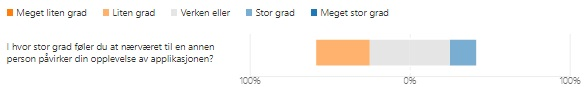
\includegraphics[width=0.9\textwidth]{fig/phase_3/survey/ValgKompAppPrecence.jpg}
 \caption{Bar chart showing the distribution of how the participants ranked according to the statement: \textit{To what degree do you feel the presence to another user affect the experience of the application}.}
\label{fig:phase3_SurveyPrecenceIncrease}
\end{figure}




Of those who tried the application (total 6 participants) half of them used the VR mode and the other half used the desktop mode. Ranking how different collaboration mechanisms worked according to their experience of using the application 50\% thought verbal communication worked to a \textit{High degree}. The other 50\% ranked it \textit{Neutral}. Interestingly, as seen in figure \ref{fig:phase3_CollabHandGestures}, 33\% (or 1/3) ranked the use of hand gesture as a communications method to a \textit{Low degree}, the median and mode being \textit{Neutral}. Also, one third ranked laser pointer to a \textit{High degree}.

As for the participants perceived understanding of what other users in the application did and planned, 16.7\% ranked it to a \textit{High degree} and the mode being \textit{Neutral} with 83.3\%. 
One third (or 33.3\%) of the participants thought the laser pointer mechanism worked to a \textit{High degree}. 
Figure \ref{fig:phase3_socialPresence} shows how the participants perceived the subjective feeling of presence (first bar) and their conscious of other users in the application (second bar). Two thirds (66.6\%) ranked \textit{High degree} related to presence, whilst half (50\%) also ranked \textit{High degree} in regards to their 
conscious of other users within the application. No one ranked it below \textit{Neutral} or higher than \textit{High degree}. 

\begin{figure}[H]
  \centering
   \captionsetup{width=.8\linewidth}
    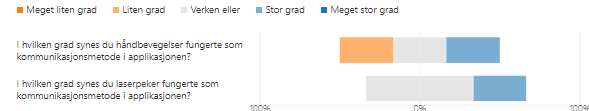
\includegraphics[width=0.9\textwidth]{fig/phase_3/survey/collabMechanisimsGestureLaser.png}
 \caption{Bar chart showing the distribution of how the participants ranked hand gesture and laser pointer as a collaboration mechanism.}
\label{fig:phase3_CollabHandGestures}
\end{figure}


\begin{figure}[H]
  \centering
   \captionsetup{width=.8\linewidth}
    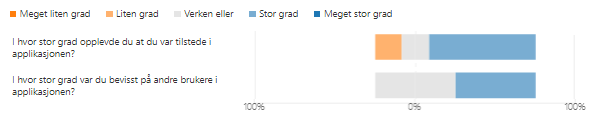
\includegraphics[width=0.9\textwidth]{fig/phase_3/survey/socialPrecense.png}
 \caption{Bar charts showing the distribution of how the participants ranked the feeling of presence and their 
conscious of other users.}
\label{fig:phase3_socialPresence}
\end{figure}


In regards to features which can facilitate the use of the application for remote carer guidance and to what degree they could be useful, the participants ranked several of them. These features included for instance verbal or written communication, ability to mark objects, and system intuitiveness. Figure \ref{fig:phase3_VerbalWritten} shows that participants heavily favoured verbal communication over written as a quality which is important for remote usage. Almost two thirds (64.7\%) ranked verbal communication as \textit{Very important} whereas none ranked in \textit{Very important} for written communication. The mode and median being \textit{Neutral}.
For qualities related to ease of use and intuitiveness the mode was \textit{Very important} for all, with an average ranking of \textit{Very important} of 72\%, which is almost three fourths of all answers.  See figure \ref{fig:phase3_Intuitiveness}.   
Additionally,  figure \ref{fig:phase3_AppBeUsed} shows the distribution of their opinions regarding whether or not the application developed in this thesis can be useful for remote career guidance. 82\% ranked either \textit{Strongly agree} or \textit{Agree}.


\begin{figure}[H]
  \centering
   \captionsetup{width=.8\linewidth}
    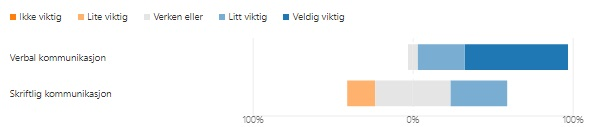
\includegraphics[width=0.9\textwidth]{fig/phase_3/survey/RemoteVerbalWritten.jpg}
 \caption{Bar chart showing the distribution of how the participants ranked verbal and written communication as useful qualities.}
\label{fig:phase3_VerbalWritten}
\end{figure}

\begin{figure}[H]
  \centering
   \captionsetup{width=.8\linewidth}
    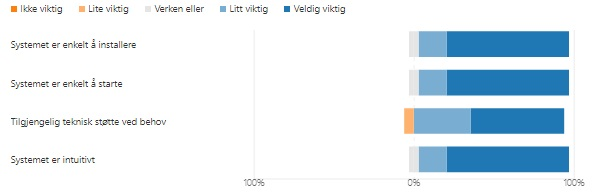
\includegraphics[width=0.9\textwidth]{fig/phase_3/survey/EaseOfUse.jpg}
 \caption{Bar chart showing the distribution of how the participants ranked statements related to intuitiveness and ease of use.}
\label{fig:phase3_Intuitiveness}
\end{figure}

\begin{figure}[H]
  \centering
   \captionsetup{width=.8\linewidth}
    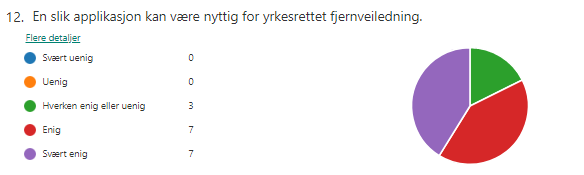
\includegraphics[width=0.9\textwidth]{fig/phase_3/survey/remoteUsage.PNG}
 \caption{Pie chart showing the distribution of how the participants ranked how useful the application can be for remote occupational guidance.}
\label{fig:phase3_AppBeUsed}
\end{figure}


The were also a strong general consensus that remote guidance in VR can be relevant for several use cases, including young job seekers, at school, as a result of geographical distance or due safety measures in workplaces. The mode for all, except one, was \textit{Very relevant} with an average of 62\%. The use case in context of unemployed as a cause of Covid-19 had the mode ranking of \textit{Somewhat relevant} being the least ranked relevant use case with 11.8\%  ranking it \textit{Less relevant}. Se figure \ref{fig:phase3_RemoteUsecases}.    

\begin{figure}[H]
  \centering
   \captionsetup{width=.8\linewidth}
    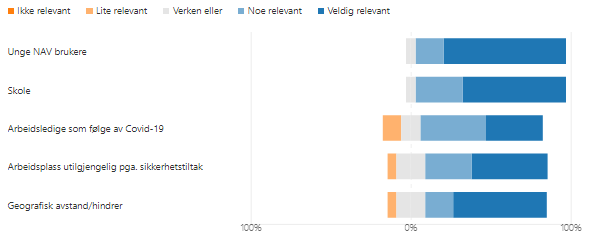
\includegraphics[width=0.9\textwidth]{fig/phase_3/survey/RemoteUseCases.PNG}
 \caption{Bar chart showing the distribution of how the participants ranked how relevant the application can be for remote VR guidance.}
\label{fig:phase3_RemoteUsecases}
\end{figure}


\subsubsection{SUS Score}
The survey contained a section for a system usability scale (SUS). To interpret the score we used the same procedure as in phase 2 (see section \ref{section:phase2SUS}). Firstly, we calculated the SUS score for each participant. There were a total of six scores as these participants were the one who had used the application during testing. The scores can be found in table \ref{table:phase3SUSscores} alongside their adjective rating and grade from table \ref{table:SUSinterpret} in phase 2.


\begin{table}[H]
\centering
\begin{tabular}{l|l|l|l}
{\textbf{Participant ID}} & { \textbf{SUS score}} & { \textbf{Grade}} & { \textbf{Adjective Rating}}\\ \hline
16   & 60   &  D & Poor                                   \\ 
2   & 62.5 &  D & Poor                                    \\ 
1   & 65 &  D & Poor                                   \\ 
15   & 65 &  D & Poor                                     \\ 
4   & 68 &  C & Okay                                    \\ 
17   & 72.5 &  B & Good                                     \\ 
\end{tabular}
\caption{SUS scores for participants sorted ascending by score.}
\label{table:phase3SUSscores}
\end{table}

This gives an average SUS score of: 
\[\overline{SUS} = \frac{60 + 65.5 + 65 + 65 + 68 + 72.5}{6} = \frac{393}{6} \approx 65.5\]

According to table \ref{table:SUSinterpret} this yields a \textit{Poor} rating of the usability of the system. As the number of individual scores are low such scales are generally prone to being volatile and effected by widespread results. However, these score were all fairly close with the range (how far apart the highest and lowest scores where) being 12.5 points. This is just a variation of a single grade in the rating. The median SUS score was 65, which correlates to the rating \textit{Poor}. This shows that there were a general consent that the usability of the system of could be improved according to the SUS method. 


\cleardoublepage